\documentclass[11pt,a4paper]{article}
\usepackage[margin=2.4cm]{geometry}
\usepackage{microtype}
\usepackage{setspace}
\usepackage{float}
\usepackage{caption}
\usepackage{hyperref}
\usepackage[table]{xcolor}
\makeatletter
\def\input@path{{.}{docs/}{./docs/}{../docs/}}
\makeatother
% shared notation and packages for slides.tex and report.tex
\usepackage{amsmath,amssymb}
\usepackage{booktabs}
\usepackage{graphicx}
\usepackage{siunitx}
\usepackage{xcolor}
\usepackage{tikz}
\usetikzlibrary{arrows.meta,positioning,shapes.geometric,calc}
\makeatletter
\providecommand{\input@path}{}
\g@addto@macro\input@path{{.}{docs/}{./docs/}{../docs/}}
\makeatother
\graphicspath{{../figures/}{figures/}{docs/figures/}}
% generated by code/12_export_tex.py -- do not edit by hand
\newcommand{\VfourMaize}{0.018}
\newcommand{\VfourPwMaize}{0.005}
\newcommand{\VfourPwRice}{0.001}
\newcommand{\VfourPwSoybean}{0.009}
\newcommand{\VfourPwWheat}{0.084}
\newcommand{\VfourRice}{0.002}
\newcommand{\VfourSoybean}{0.008}
\newcommand{\VfourWheat}{0.065}
\newcommand{\adqYears}{2021--2023}
\newcommand{\bTMaizeSAfrica}{-27.8}
\newcommand{\bTMaizeUSA}{-6.4}
\newcommand{\bTRiceIndia}{-11.4}
\newcommand{\bTWheatIndia}{-4.2}
\newcommand{\bWMaizeSAfrica}{+0.0}
\newcommand{\bWMaizeUSA}{+0.0}
\newcommand{\bWRiceIndia}{+0.0}
\newcommand{\bWWheatIndia}{+0.0}
\newcommand{\bdRiceKcal}{63}
\newcommand{\bdRiceZinc}{55}
\newcommand{\bdShockKcal}{-6.3}
\newcommand{\bdShockKcalAbs}{6.3}
\newcommand{\bdShockMar}{-0.50}
\newcommand{\egWheatIron}{46}
\newcommand{\egWheatKcal}{34}
\newcommand{\egWheatSone}{-3.6}
\newcommand{\egWheatZinc}{48}
\newcommand{\exEheat}{1.00}
\newcommand{\exEwater}{0.33}
\newcommand{\exI}{0.222}
\newcommand{\exImax}{0.421}
\newcommand{\exIn}{0.53}
\newcommand{\exLheat}{0.58}
\newcommand{\exLwater}{17.8}
\newcommand{\exSheat}{0.43}
\newcommand{\exShlit}{0.50}
\newcommand{\exShobs}{0.36}
\newcommand{\exSwater}{0.44}
\newcommand{\exSwlit}{0.88}
\newcommand{\exSwobs}{0.00}
\newcommand{\exVfour}{0.151}
\newcommand{\feRatioBangladesh}{0.70}
\newcommand{\feRatioBrazil}{0.97}
\newcommand{\feRatioEgypt}{1.20}
\newcommand{\feRatioIndia}{0.89}
\newcommand{\feRatioNigeria}{0.91}
\newcommand{\feRatioRussia}{1.14}
\newcommand{\feRatioSAfrica}{0.82}
\newcommand{\heatCellsMaize}{7}
\newcommand{\heatCellsRice}{2}
\newcommand{\heatCellsSoybean}{0}
\newcommand{\heatCellsWheat}{22}
\newcommand{\inRiceSone}{-4.8}
\newcommand{\inWheatKcal}{-2.1}
\newcommand{\inWheatMar}{-0.52}
\newcommand{\inWheatMarTrade}{-0.28}
\newcommand{\koppenAgree}{93}
\newcommand{\koppenAgreeMaize}{92}
\newcommand{\koppenAgreeRice}{93}
\newcommand{\koppenAgreeSoybean}{95}
\newcommand{\koppenAgreeWheat}{83}
\newcommand{\maizeFeedBrazil}{75}
\newcommand{\maizeFeedChina}{72}
\newcommand{\maizeFeedUS}{46}
\newcommand{\maizeFeedWorld}{60}
\newcommand{\maizeFoodSAfrica}{40}
\newcommand{\maizeFoodWorld}{12}
\newcommand{\marBangladesh}{0.939}
\newcommand{\marBrazil}{0.994}
\newcommand{\marEgypt}{1.000}
\newcommand{\marIndia}{0.978}
\newcommand{\marNigeria}{0.981}
\newcommand{\marRussia}{1.000}
\newcommand{\marSAfrica}{0.964}
\newcommand{\mcFourMaizeFirst}{1.0}
\newcommand{\mcFourRiceFirst}{0.0}
\newcommand{\mcFourSoybeanFirst}{1.5}
\newcommand{\mcFourWheatFirst}{97.5}
\newcommand{\mcOneMaizeFirst}{1.0}
\newcommand{\mcOneRiceFirst}{0.0}
\newcommand{\mcOneSoybeanFirst}{1.3}
\newcommand{\mcOneWheatFirst}{97.7}
\newcommand{\nCountriesAdq}{205}
\newcommand{\nPassNew}{26}
\newcommand{\nPassNewSig}{1}
\newcommand{\nPassOld}{26}
\newcommand{\nPassOldSig}{9}
\newcommand{\nRobustT}{7}
\newcommand{\nRobustW}{5}
\newcommand{\nShared}{5}
\newcommand{\nShock}{26}
\newcommand{\orderFour}{Wheat $>$ Maize $>$ Soybean $>$ Rice}
\newcommand{\orderFourPw}{Wheat $>$ Soybean $>$ Maize $>$ Rice}
\newcommand{\orderOne}{Wheat $>$ Maize $>$ Soybean $>$ Rice}
\newcommand{\pShock}{0.170}
\newcommand{\pShockE}{0.169}
\newcommand{\pShockS}{0.467}
\newcommand{\panelShareMaize}{69}
\newcommand{\panelShareRice}{63}
\newcommand{\panelShareSoybean}{90}
\newcommand{\panelShareWheat}{51}
\newcommand{\passRiceBangladesh}{0.37}
\newcommand{\passRiceChina}{0.90}
\newcommand{\passRiceIndia}{0.37}
\newcommand{\passSoyHi}{1.8}
\newcommand{\passSoyLo}{1.6}
\newcommand{\poolTMaize}{-11.7}
\newcommand{\poolTRice}{-1.1}
\newcommand{\poolTSoybean}{-6.2}
\newcommand{\poolTWheat}{-2.7}
\newcommand{\poolTpMaize}{0.000}
\newcommand{\poolTpRice}{0.476}
\newcommand{\poolTpSoybean}{0.000}
\newcommand{\poolTpWheat}{0.019}
\newcommand{\poolWMaize}{+1.5}
\newcommand{\poolWRice}{+0.3}
\newcommand{\poolWSoybean}{+1.8}
\newcommand{\poolWWheat}{-2.4}
\newcommand{\poolWpMaize}{0.079}
\newcommand{\poolWpRice}{0.422}
\newcommand{\poolWpSoybean}{0.020}
\newcommand{\poolWpWheat}{0.080}
\newcommand{\pshareIronMaize}{8.3}
\newcommand{\pshareIronRice}{9.4}
\newcommand{\pshareIronSoybean}{1.2}
\newcommand{\pshareIronWheat}{32.8}
\newcommand{\pshareProteinMaize}{5.1}
\newcommand{\pshareProteinRice}{13.4}
\newcommand{\pshareProteinSoybean}{0.6}
\newcommand{\pshareProteinWheat}{21.9}
\newcommand{\pshareZincMaize}{7.6}
\newcommand{\pshareZincRice}{15.3}
\newcommand{\pshareZincSoybean}{0.5}
\newcommand{\pshareZincWheat}{32.5}
\newcommand{\rankFourMaize}{2}
\newcommand{\rankFourPwMaize}{3}
\newcommand{\rankFourPwRice}{4}
\newcommand{\rankFourPwSoybean}{2}
\newcommand{\rankFourPwWheat}{1}
\newcommand{\rankFourRice}{4}
\newcommand{\rankFourSoybean}{3}
\newcommand{\rankFourWheat}{1}
\newcommand{\rhoShock}{+0.20}
\newcommand{\rhoShockE}{+0.19}
\newcommand{\rhoShockS}{+0.02}
\newcommand{\rhoZhaoClim}{+0.8}
\newcommand{\rhoZhaoFour}{+0.6}
\newcommand{\rhoZhaoFourPw}{+0.0}
\newcommand{\rhoZhaoHeat}{+0.8}
\newcommand{\rhoZhaoOne}{+0.6}
\newcommand{\rhoZhaoPool}{+0.4}
\newcommand{\riskIronMaize}{0.48}
\newcommand{\riskIronRice}{0.49}
\newcommand{\riskIronSoybean}{0.05}
\newcommand{\riskIronWheat}{1.67}
\newcommand{\riskProteinMaize}{0.00}
\newcommand{\riskProteinRice}{1.05}
\newcommand{\riskProteinSoybean}{0.00}
\newcommand{\riskProteinWheat}{1.38}
\newcommand{\riskZincMaize}{0.00}
\newcommand{\riskZincRice}{0.51}
\newcommand{\riskZincSoybean}{0.02}
\newcommand{\riskZincWheat}{3.02}
\newcommand{\robN}{80}
\newcommand{\robWheatTopAll}{80}
\newcommand{\rtwoMaize}{0.24}
\newcommand{\rtwoMaxMaize}{0.50}
\newcommand{\rtwoMaxRice}{0.26}
\newcommand{\rtwoMaxSoybean}{0.54}
\newcommand{\rtwoMaxWheat}{0.22}
\newcommand{\rtwoMinMaize}{0.05}
\newcommand{\rtwoMinRice}{0.01}
\newcommand{\rtwoMinSoybean}{0.05}
\newcommand{\rtwoMinWheat}{0.02}
\newcommand{\rtwoRice}{0.04}
\newcommand{\rtwoSoybean}{0.17}
\newcommand{\rtwoWheat}{0.13}
\newcommand{\saMaizeSone}{-26.8}
\newcommand{\sharedPanel}{Brazil, China, India, Russia, USA}
\newcommand{\sharedWheatTop}{5}
\newcommand{\skillMedian}{0.31}
\newcommand{\skillN}{21}
\newcommand{\skillPos}{18}
\newcommand{\snrHeatMaize}{0.68}
\newcommand{\snrHeatRice}{0.92}
\newcommand{\snrHeatSoybean}{0.64}
\newcommand{\snrHeatWheat}{0.80}
\newcommand{\soyFoodWorld}{4}
\newcommand{\soyProcChina}{81}
\newcommand{\soyProcUS}{92}
\newcommand{\soyProcWorld}{86}
\newcommand{\tauOneFour}{0.91}
\newcommand{\tauOneThree}{0.58}
\newcommand{\worldFatMaize}{1.4}
\newcommand{\worldFatRice}{1.8}
\newcommand{\worldFatSoybean}{12.5}
\newcommand{\worldFatWheat}{3.5}
\newcommand{\worldIMaize}{4.2}
\newcommand{\worldIRice}{10.2}
\newcommand{\worldISoybean}{4.5}
\newcommand{\worldIWheat}{18.7}
\newcommand{\worldIronMaize}{5.6}
\newcommand{\worldIronRice}{7.6}
\newcommand{\worldIronSoybean}{3.3}
\newcommand{\worldIronWheat}{26.0}
\newcommand{\worldKcalMaize}{4.9}
\newcommand{\worldKcalRice}{17.1}
\newcommand{\worldKcalSoybean}{3.7}
\newcommand{\worldKcalWheat}{17.8}
\newcommand{\worldProteinMaize}{3.3}
\newcommand{\worldProteinRice}{11.4}
\newcommand{\worldProteinSoybean}{1.8}
\newcommand{\worldProteinWheat}{18.8}
\newcommand{\worldZincMaize}{5.8}
\newcommand{\worldZincRice}{13.1}
\newcommand{\worldZincSoybean}{1.3}
\newcommand{\worldZincWheat}{27.2}
\newcommand{\worstMar}{-0.53}
\newcommand{\worstMarCase}{Maize in S. Africa}



\definecolor{rice}{HTML}{2A7F62}
\definecolor{wheat}{HTML}{C8961A}
\definecolor{maize}{HTML}{C0504D}
\definecolor{soy}{HTML}{5B5EA6}
\definecolor{ink}{HTML}{222222}
\definecolor{muted}{HTML}{6B6B6B}
\definecolor{paddy}{HTML}{1F4E3D}
\definecolor{grain}{HTML}{C8961A}
\definecolor{clay}{HTML}{B5523B}
\newcommand{\Teff}{T_{\mathrm{eff}}}
\newcommand{\Tcrit}{T_{\mathrm{crit}}}
\newcommand{\ETc}{\mathrm{ET_c}}
\newcommand{\ETo}{\mathrm{ET_0}}
\usepackage{adjustbox}


\usepackage[round]{natbib}
\usepackage{booktabs}
\bibliographystyle{plainnat}
\let\parencite\citep
\let\textcite\citet
\hypersetup{colorlinks=true,linkcolor=paddy,citecolor=paddy,urlcolor=paddy}
\captionsetup{font=small,labelfont=bf}
\setstretch{1.08}
\setlength{\parskip}{0.45em}
\setlength{\parindent}{0pt}
\newcommand{\TT}{\mathrm{T}}   % temperature
\newcommand{\PP}{\mathrm{P}}   % precipitation

\title{\textbf{Climate Change and Nutritional Security:\\ Which Crops Are Most Vulnerable?}\\[0.4em]
\large Mid-evaluation report: a Climate--Nutrition Vulnerability Index for rice, wheat, maize and soybean}
\author{Arpit Mahtele \and Dev Patel \and Navey Puri \and Shreyash Lohare}
\date{Earth 616 \quad $\cdot$ \quad observed data 1971--2024}

\begin{document}
\maketitle

\begin{abstract}\small
We build an index of crop vulnerability that combines how strongly a crop's growing areas are exposed to heat and water stress (\emph{Exposure}), how much yield is lost per unit of that stress (\emph{Sensitivity}), and how much of a population's energy, protein, fat, zinc and iron the crop supplies (\emph{Importance}). It is applied to rice, wheat, maize and soybean with observed climate from 1971 to 2024, across major producing countries in different climate zones (USA, Brazil, India, China, Russia, South Africa, Bangladesh, Egypt, Nigeria, Argentina). Sensitivity is parameterized directly from established crop literature (heat damage thresholds and FAO yield response factors $K_y$), providing a standardized per-crop response scale. Wheat emerges as the most vulnerable crop under all candidate index formulas in the main run (\orderFour\ with equal weights, \orderFourPw\ production-weighted) and in \robWheatTopAll{} of \robN{} robustness rankings. Wheat leads through high nutritional Importance (supplying the majority of cereal protein, zinc and iron) and substantial climate exposure; maize and soybean are more sensitive to heat per \si{\celsius} but are largely used for feed or processing rather than direct human food. Rice scores lowest because it is predominantly irrigated and monthly flowering-season temperatures remain below its \SI{35}{\celsius} critical limit on gridded monthly averages. A standard 10\% yield loss reduces the Mean Adequacy Ratio (MAR) most severely where iron supply is already marginal. All figures and tables in this document are generated directly from the analysis pipeline.
\end{abstract}

\tableofcontents
\newpage

% =====================================================================
\section{Problem statement}
Climate change affects food security through two channels: how much of each crop is produced, and what that crop contributes nutritionally. Most published literature addresses only one of these channels: climate explains about a third of global yield variability \parencite{ray2015}, and warming lowers global yields of wheat, rice, maize and soybean by about 6.0, 3.2, 7.4 and 3.1\% per \si{\celsius} \parencite{zhao2017}. Elevated CO$_2$ lowers zinc, iron and protein in C3 crops \parencite{myers2014,smith2018}, a separate line of research. Because published metrics operate on incompatible scales, no previous study ranks crops by combining climatic exposure, crop sensitivity, and nutritional importance into a unified index.

This report documents our Climate--Nutrition Vulnerability Index (CNVI) framework, its data inputs, calculations, and findings. It addresses two core questions:
\begin{enumerate}
\item Which of the four crops is most vulnerable to observed changes in temperature and rainfall, once we also account for dietary importance?
\item If a crop's yield falls, what happens to a country's nutrient supply and adequacy?
\end{enumerate}
The framework adapts the IPCC risk structure ($\text{Vulnerability} = \text{Exposure} \times \text{Sensitivity} \times \text{Importance}$), where \emph{adaptive capacity} is replaced by \emph{nutritional importance}, focusing explicitly on nutritional security at the population level.

% =====================================================================
\section{Data}
\begin{table}[H]\centering\scriptsize
\begin{tabular}{p{3.3cm}p{4.3cm}p{1.8cm}p{3.6cm}}
\toprule
Dataset & Content & Period & Used for\\
\midrule
WorldClim 2.1 historical monthly weather (CRU-TS 4.09 downscaled), 10$'$ \parencite{fick2017,harris2020} & monthly Tmax, Tmin, precipitation & 1970--2024 & hazards, K\"oppen class\\
SPAM 2010 v2.0 \parencite{spam2010} & harvested area per crop, irrigated / rainfed, 5$'$ & c.\,2010 & area weights, rainfed share\\
Sacks et al.\ crop calendar \parencite{sacks2010} & planting and harvest day per cell & climatology & growing and flowering windows\\
FAOSTAT crops (QCL) \parencite{faostat} & production, area, yield by country & 1961--2024 & panels, out-of-sample data check\\
FAOSTAT Food Balances 2010-- and $-$2013 & kcal, protein, fat, food quantity per item & 2010--23; 1961--2013 & Importance, adequacy, pass-through\\
FAOSTAT food-security indicators & Average Dietary Energy Requirement & 2000--23 & energy requirement\\
USDA FoodData Central, SR Legacy \parencite{usda2019} & zinc, iron per 100\,g & 2018 & zinc and iron supply\\
Natural Earth 1:50\,m & borders, continents & static & country masks\\
\bottomrule
\end{tabular}
\caption{Datasets used in the analysis pipeline (downloaded by \texttt{code/01\_download\_data.py}; details in \texttt{docs/DATA\_SOURCES.md}).}
\end{table}

\textbf{Why monthly weather and not normals.} A 30-year normal cannot show variability, change or the frequency of bad seasons. Year-by-year data capture observed stress conditions. \textbf{Why SPAM and the Sacks calendar.} National averages mix crop areas with unsuitable terrain; grid-cell crop areas and specific growing calendars ensure climate metrics reflect where and when each crop is actually cultivated. \textbf{Food balances.} The 1961--2013 and 2010--2023 FAOSTAT series are analysed separately due to methodological breaks.

% =====================================================================
\section{Methodology}
\subsection{Country panels}
Country panels were selected systematically:
\begin{enumerate}
\item \textbf{Core countries:} USA, Brazil, India and China for all four crops.
\item \textbf{Regional representation:} One European and one African country per crop. Russia represents Europe (ranking in Europe's top-3 producers for all four crops). In Africa, top producers vary: Nigeria for rice, Egypt for wheat, South Africa for maize and soybean.
\item \textbf{World top-3 producers:} Adds Bangladesh for rice and Argentina for soybean.
\end{enumerate}
The panels cover \panelShareRice\% (rice), \panelShareWheat\% (wheat), \panelShareMaize\% (maize) and \panelShareSoybean\% (soybean) of global production.

\begin{table}[H]\centering\scriptsize
\begin{tabular}{llrrlrl}
\toprule
Crop & Country & Rank & Share (\%) & Class & Elev. (m) & Crop area in A/B/C/D (\%)\\
\midrule
Rice & China & 1 & 26.4 & C & 260 & 1/1/86/12 \\
 & India & 2 & 25.1 & A & 216 & 51/12/37/0 \\
 & Bangladesh & 3 & 7.4 & A & 17 & 62/0/38/0 \\
 & Brazil & 11 & 1.4 & A & 208 & 53/0/47/0 \\
 & USA & 13 & 1.2 & C & 52 & 0/0/100/0 \\
 & Nigeria & 14 & 1.1 & A & 368 & 89/11/0/0 \\
 & Russia & 39 & 0.1 & C & 21 & 0/10/52/38 \\
\midrule
Wheat & China & 1 & 17.3 & C & 386 & 0/22/51/27 \\
 & India & 2 & 13.9 & C & 255 & 14/34/52/0 \\
 & Russia & 3 & 11.2 & D & 177 & 0/1/2/97 \\
 & USA & 4 & 6.1 & D & 647 & 0/31/24/44 \\
 & Egypt & 17 & 1.2 & B & 42 & 0/100/0/0 \\
 & Brazil & 19 & 1.0 & C & 567 & 5/0/95/0 \\
\midrule
Maize & USA & 1 & 31.0 & D & 361 & 0/6/12/83 \\
 & China & 2 & 23.3 & D & 429 & 0/20/28/52 \\
 & Brazil & 3 & 9.2 & A & 512 & 53/6/41/0 \\
 & India & 5 & 2.9 & A & 435 & 37/30/31/1 \\
 & S. Africa & 8 & 1.3 & B+M & 1400 & 0/52/48/0 \\
 & Russia & 9 & 1.2 & D & 155 & 0/1/12/87 \\
\midrule
Soybean & Brazil & 1 & 36.4 & A & 531 & 59/0/41/0 \\
 & USA & 2 & 31.5 & D & 278 & 0/0/22/77 \\
 & Argentina & 3 & 11.4 & C & 159 & 0/6/94/0 \\
 & China & 4 & 5.3 & D & 333 & 0/6/33/61 \\
 & India & 5 & 3.7 & A & 420 & 70/10/20/0 \\
 & Russia & 8 & 1.6 & D & 152 & 0/0/4/96 \\
 & S. Africa & 12 & 0.5 & C+M & 1273 & 1/45/55/0 \\
\bottomrule
\end{tabular}

\caption{Country panels. Rank: global production rank; Share: \% of world production; Class: primary K\"oppen group (+M for mountain elevation $\ge 1000$\,m).}\label{tab:panels}
\end{table}

\begin{figure}[H]\centering
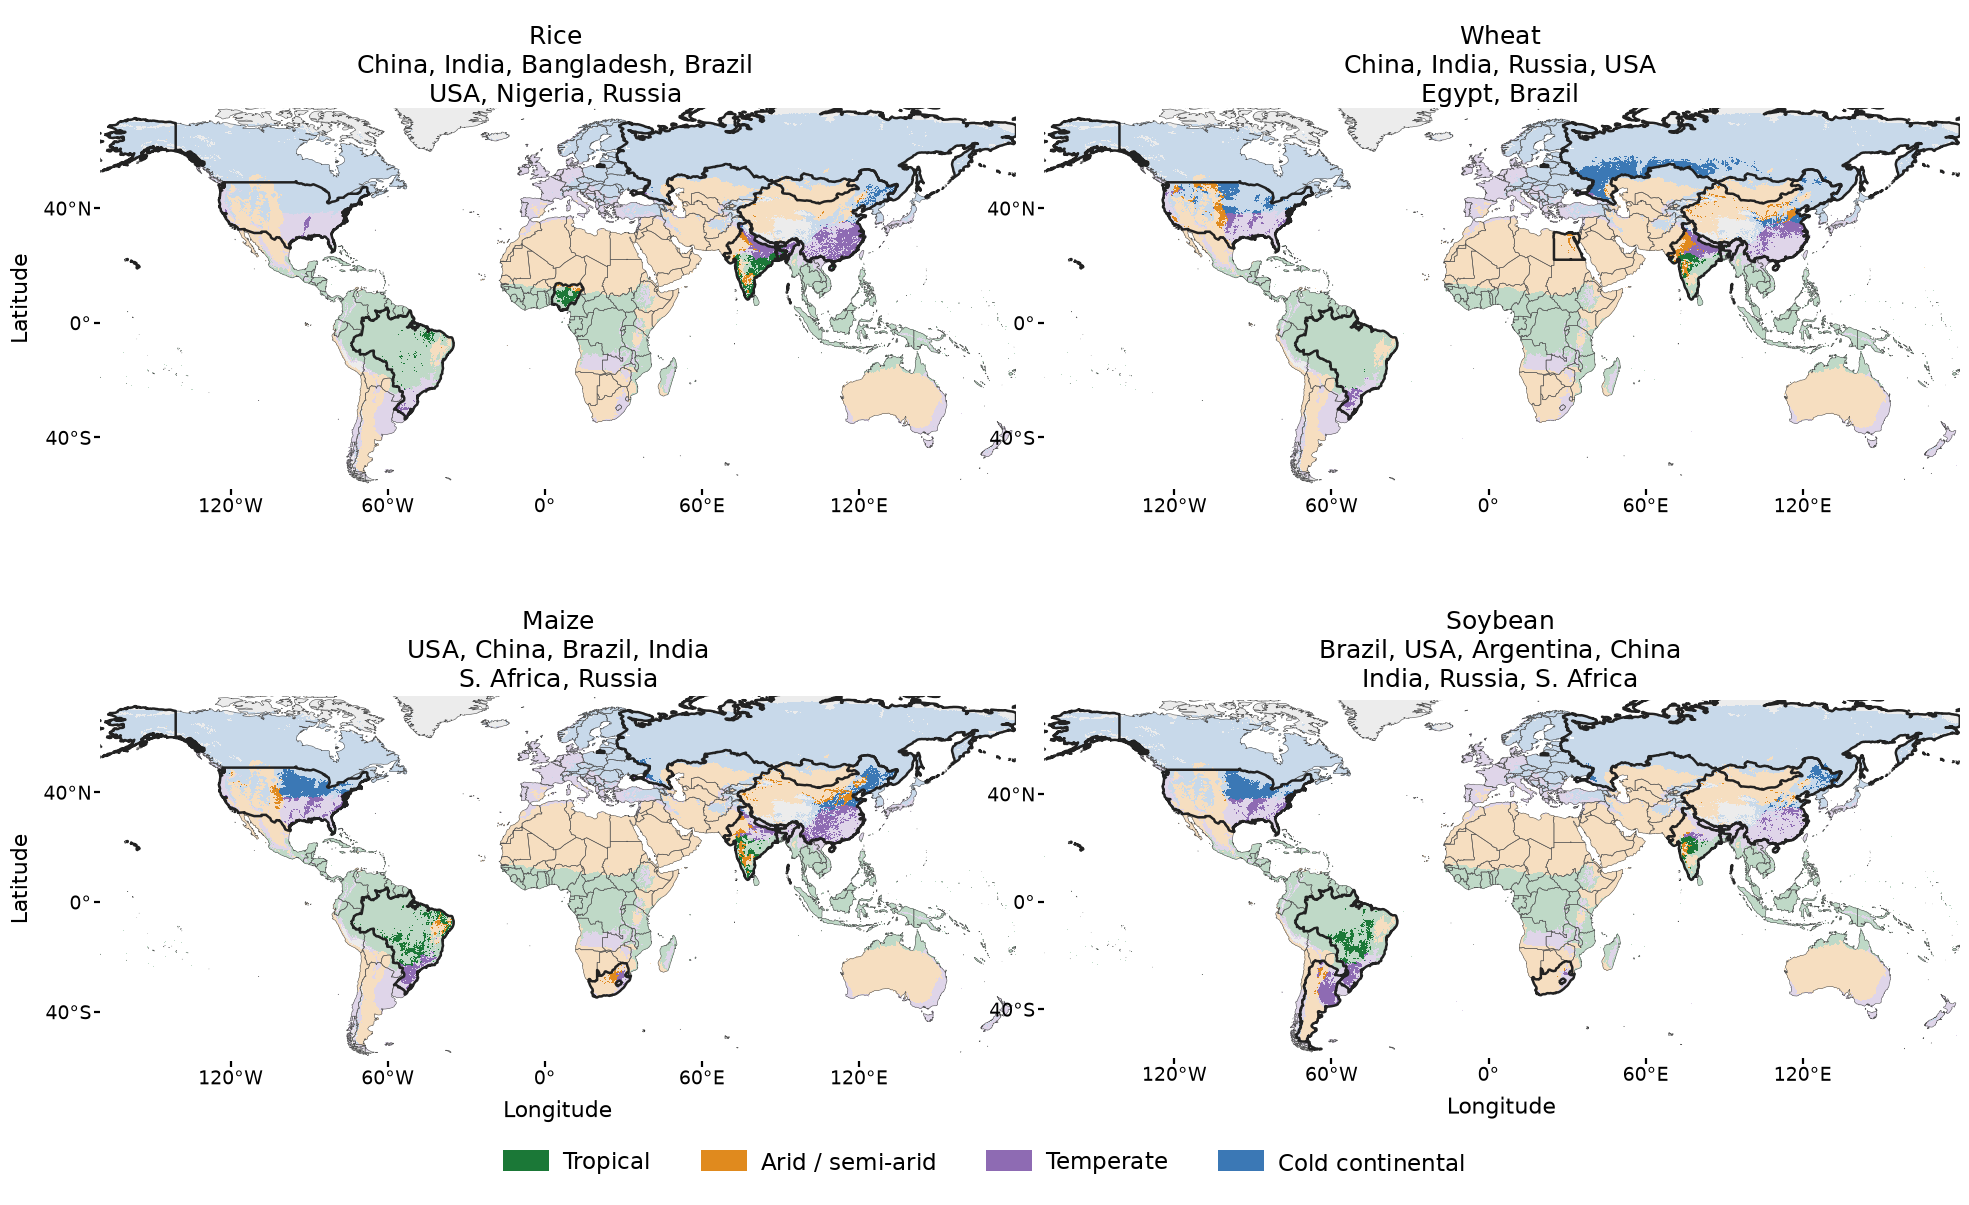
\includegraphics[width=\linewidth]{F01_panels_koppen.png}
\caption{Panel countries (black outlines) and climate classes where each crop grows across K\"oppen zones (A: tropical, B: arid, C: temperate, D: cold continental).}
\end{figure}

\subsection{Exposure}
Exposure measures the physical climate stress experienced by crop growing areas over 2001--2024, evaluated across temperature (heat) and precipitation (water).

\paragraph{Temperature Exposure ($E^{\TT}$).} Heat damage concentrates during the reproductive flowering phase (anthesis). Following \textcite{deryng2014}, flowering occurs during 45--70\% of the growing season length. Heat stress level $L^{\TT}$ measures the degrees by which effective temperature $T_{eff} = \tfrac12(T_{mean}+T_{max})$ exceeds the crop critical limit $T_{crit}$:
\begin{equation}
E^{\TT} = \frac{L^{\TT}}{\max L^{\TT}},\qquad L^{\TT} = \operatorname*{mean}_{2001\text{--}24}\ \frac{\sum_m w_m \max(0,\; T_{eff,m} - T_{crit})}{\sum_m w_m}
\end{equation}
where $w_m$ is the fraction of month $m$ inside the flowering window. Critical limits are: wheat \SI{25}{\celsius}, maize \SI{32}{\celsius}, soybean \SI{35}{\celsius} \parencite{deryng2014}, and rice \SI{35}{\celsius} \parencite{yoshida1981,fao66}. $E^{\TT}$ is normalized to 0--1 across all crop--country pairs by dividing by the maximum observed level ($\max L^{\TT}$).

\paragraph{Precipitation Exposure ($E^{\PP}$).} Water stress measures the share of crop water requirements unmet by rainfall on rainfed hectares:
\begin{equation}
E^{\PP} = \frac{L^{\PP}}{\max L^{\PP}},\qquad L^{\PP} = \operatorname*{mean}_{2001\text{--}24}\ \frac{\sum_{cells} R\,\max(0,\; 1 - P/ET_c)}{\sum_{cells} A}
\end{equation}
where $P$ is growing-season precipitation, $ET_c = \bar{K}_c ET_0$ is crop water demand \parencite{fao56}, $R$ is rainfed harvested hectares, and $A$ is total harvested hectares. Irrigated land is treated as having no water shortfall ($1 - P/ET_c = 0$). Reference evapotranspiration $ET_0$ is calculated using the Hargreaves equation \parencite[FAO-56 Eq.~52]{fao56} with extraterrestrial radiation $R_a$. $E^{\PP}$ is normalized to 0--1 by dividing by $\max L^{\PP}$.

\subsection{Sensitivity}
Sensitivity represents the fraction of yield lost per unit of climate stress, derived directly from established agronomic literature to ensure comparability across crops.

\paragraph{Temperature Sensitivity ($S^{\TT}$).} Based on the linear yield loss function of \textcite{deryng2014}, yield declines linearly from zero loss at $T_{crit}$ to complete loss at $T_{lim}$:
\begin{equation}
S^{\TT} = \frac{s^{\TT}}{\max s^{\TT}},\qquad s^{\TT} = \frac{1}{T_{lim} - T_{crit}}
\end{equation}
For rice, $s^{\TT} = 0.07$ per \si{\celsius} above $T_{crit}=\SI{35}{\celsius}$ based on spikelet sterility measurements from \textcite{jagadish2007} and \textcite{yoshida1981}. The values are normalized by the maximum slope ($\max s^{\TT} = 0.20$ for soybean):
\begin{itemize}\setlength{\itemsep}{1pt}
\item Soybean: $s^{\TT} = 1/(40-35) = 0.200 \implies S^{\TT} = 1.00$
\item Wheat: $s^{\TT} = 1/(35-25) = 0.100 \implies S^{\TT} = 0.50$
\item Maize: $s^{\TT} = 1/(45-32) = 0.077 \implies S^{\TT} = 0.38$
\item Rice: $s^{\TT} = 0.070 \implies S^{\TT} = 0.35$
\end{itemize}

\paragraph{Precipitation Sensitivity ($S^{\PP}$).} Based on the FAO yield response factor $K_y$ \parencite{fao66}, which relates relative yield loss to relative evapotranspiration deficit:
\begin{equation}
S^{\PP} = \frac{K_y}{\max K_y}
\end{equation}
$K_y$ values are: maize 1.25, wheat 1.10 (average of spring 1.15 and winter 1.05), soybean 0.85, and rice 1.25 \parencite{fao66,brouwer1986}. Normalized by $\max K_y = 1.25$:
\begin{itemize}\setlength{\itemsep}{1pt}
\item Rice \& Maize: $K_y = 1.25 \implies S^{\PP} = 1.00$
\item Wheat: $K_y = 1.10 \implies S^{\PP} = 0.88$
\item Soybean: $K_y = 0.85 \implies S^{\PP} = 0.68$
\end{itemize}

\begin{table}[H]\centering\small
\begin{tabular}{llcccll}
\toprule
Crop & Path & $T_{crit}/T_{lim}$ (\si{\celsius}) & $s^{lit}_{heat}$ (per \si{\celsius}) & $K_y$ & $K_c$ ini/mid/end & $\bar K_c$\\
\midrule
Rice & C3 & 35 / -- & 0.070 & 1.25 & 1.05/1.20/0.75 & 1.11 \\
Wheat & C3 & 25 / 35 & 0.100 & 1.10 & 0.40/1.15/0.33 & 0.88 \\
Maize & C4 & 32 / 45 & 0.077 & 1.25 & 0.30/1.20/0.48 & 0.84 \\
Soybean & C3 & 35 / 40 & 0.200 & 0.85 & 0.40/1.15/0.50 & 0.89 \\
\bottomrule
\end{tabular}

\caption{Literature parameters used for Exposure and Sensitivity. $T_{crit}, T_{lim}$: critical and limit temperatures; $s^{\TT}$: heat loss slope; $K_y$: FAO water yield factor; $K_c$: crop coefficients.}\label{tab:params}
\end{table}

\paragraph{Empirical Yield Regressions (Out-of-Sample Check).} Country-level regressions of detrended yield anomalies on climate variables ($y_t = a + b_T T_{eff,t} + b_W (P/ET_c)_t + \varepsilon_t$ over 1971--2000) are retained exclusively as an empirical validation check against literature benchmarks (e.g. \citealt{zhao2017}), rather than being merged into the sensitivity score.

\subsection{Importance and Nutrient Adequacy}
Dietary Importance ($I$) measures the population's nutritional reliance on each crop across five key nutritional dimensions:
\begin{equation}
I_{kc} = \frac{1}{5} \sum_{n \in \{\mathrm{kcal,\,protein,\,fat,\,Zn,\,Fe}\}} \frac{\text{supply}_n\text{ from crop }k}{\text{total national supply}_n}\qquad (2021\text{--}23\text{ mean})
\end{equation}
Calories, protein, and fat come from FAO Food Balance Sheets; zinc and iron are computed by mapping each of the 98 FBS food items to USDA FoodData Central composition values.

\paragraph{Nutrient Adequacy.} Adequacy is evaluated via the Nutrient Adequacy Ratio (NAR) and Mean Adequacy Ratio (MAR):
\begin{equation}
\mathrm{NAR}_n = \min\left(1,\; \frac{\text{supply}_n}{\text{requirement}_n}\right),\qquad \mathrm{MAR} = \frac{1}{5}\sum_{n} \mathrm{NAR}_n
\end{equation}
Truncating $\mathrm{NAR}_n$ at 1 ensures surplus in one nutrient cannot mask deficiency in another. Requirements follow WHO/FAO standards: energy from FAOSTAT Average Dietary Energy Requirement, protein at 10\% and fat at 15\% of daily energy \parencite{who2003}, zinc at \SI{11.9}{mg/day} (low bioavailability), and iron at \SI{21.6}{mg/day} (10\% bioavailability) \parencite{whofao2004}.

\subsection{Index Formulation and Candidate Forms}
For crop $k$ in country $c$, four mathematical aggregation formulas were evaluated:
\begin{align}
\text{F1 Multiplicative:}&\quad V = E \cdot S \cdot I, & E &= \tfrac12(E^{\TT}+E^{\PP}),\quad S = \tfrac12(S^{\TT}+S^{\PP})\\
\text{F2 Geometric:}&\quad V = (E \cdot S \cdot I)^{1/3}\\
\text{F3 Additive:}&\quad V = (E + S + I)/3\\
\textbf{F4 Hazard-Paired:}&\quad V = \tfrac12\big(E^{\TT}S^{\TT} + E^{\PP}S^{\PP}\big)\,I
\end{align}
\textbf{Formula F4 was chosen for fundamental design reasons:}
\begin{enumerate}
\item \emph{Hazard-specific coupling:} Each climate hazard multiplies its own corresponding sensitivity ($E^{\TT}S^{\TT}$ and $E^{\PP}S^{\PP}$). In F1--F3, high heat exposure can erroneously multiply water sensitivity.
\item \emph{No non-food vulnerability:} If a crop contributes negligibly to direct diet ($I \approx 0$), its nutritional vulnerability remains zero. Additive forms (F3) allow climate exposure alone to produce high vulnerability for non-food crops.
\item \emph{Physical interpretability:} The term $\tfrac12(E^{\TT}S^{\TT} + E^{\PP}S^{\PP})$ corresponds to expected proportional yield loss from combined climate stresses.
\end{enumerate}

% =====================================================================
\section{Results}
\subsection{Climate Exposure}
\begin{figure}[H]\centering
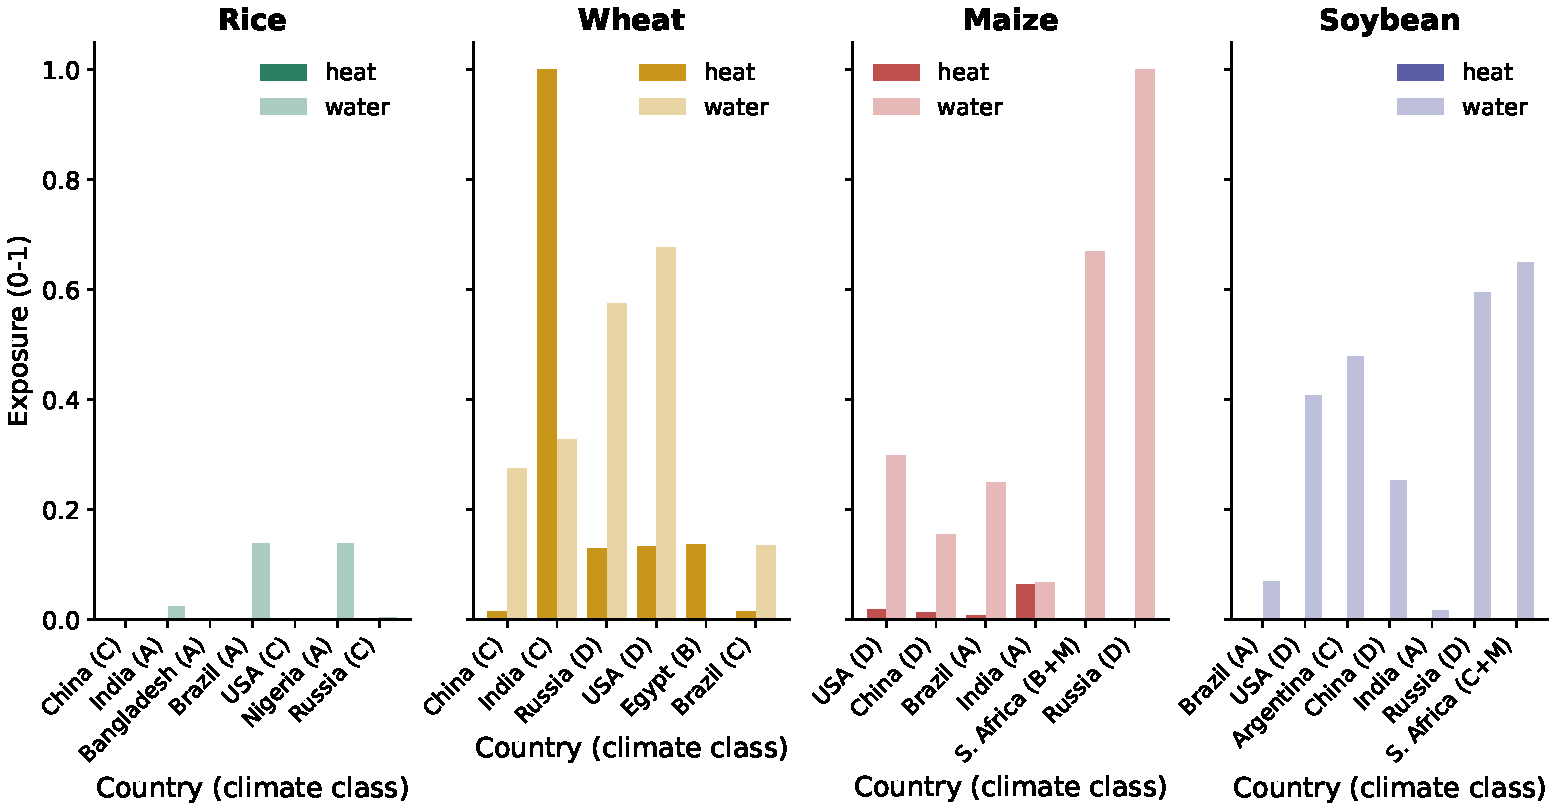
\includegraphics[width=\linewidth]{F04_exposure_by_country.pdf}
\caption{Exposure scores (0--1) by crop and country: temperature exposure $E^{\TT}$ (dark) and precipitation exposure $E^{\PP}$ (light).}
\end{figure}
Heat exposure peaks for wheat in India ($E^{\TT} = \exEheat$) due to hot conditions exceeding \SI{25}{\celsius} during anthesis. Water exposure is highest for rainfed maize in South Africa and Russia, and wheat in the USA and Russia. Rice exhibits low exposure across both dimensions ($E^{\TT} < 0.001$, $E^{\PP} < 0.14$) because major paddies are heavily irrigated and monthly averages do not exceed \SI{35}{\celsius}.

\subsection{Nutritional Importance and Adequacy}
\begin{figure}[H]\centering
\begin{minipage}{0.49\textwidth}
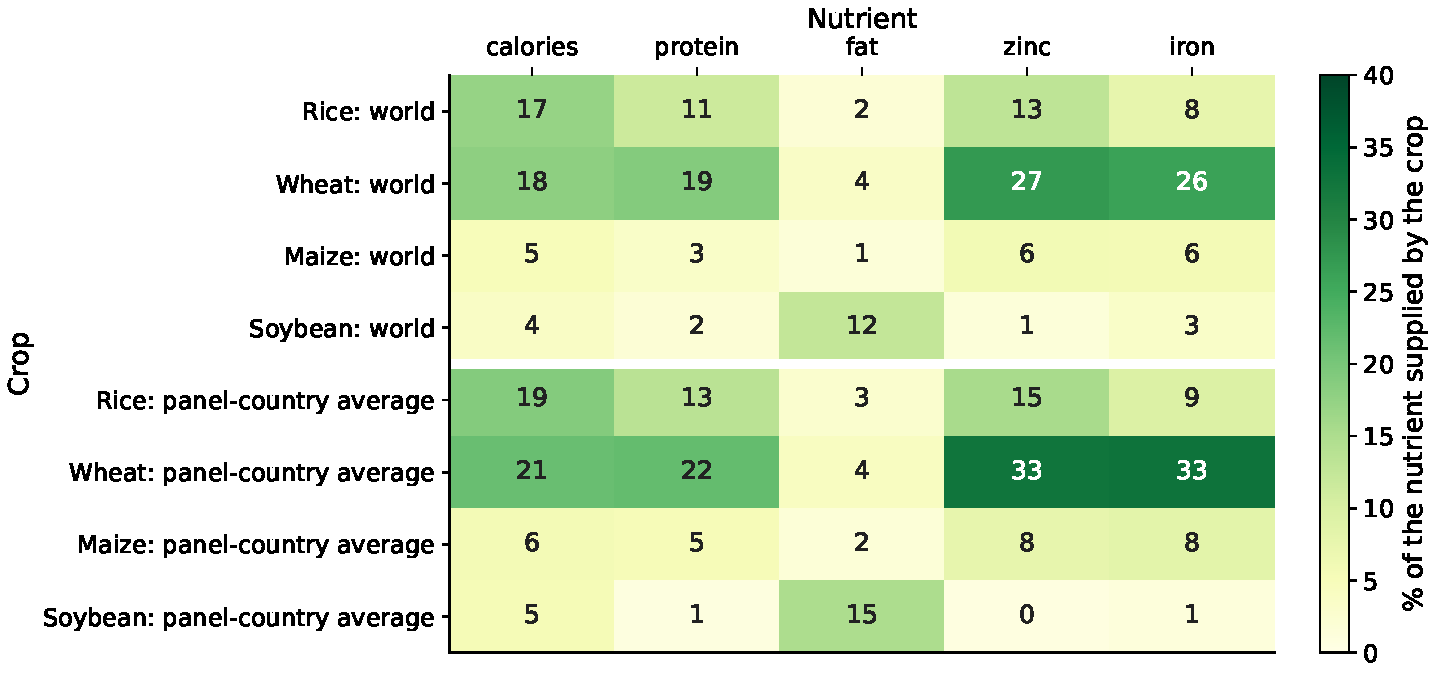
\includegraphics[width=\linewidth]{F06s_importance_summary.pdf}
\caption{Nutritional supply share (\%) by crop.}
\end{minipage}\hfill
\begin{minipage}{0.49\textwidth}
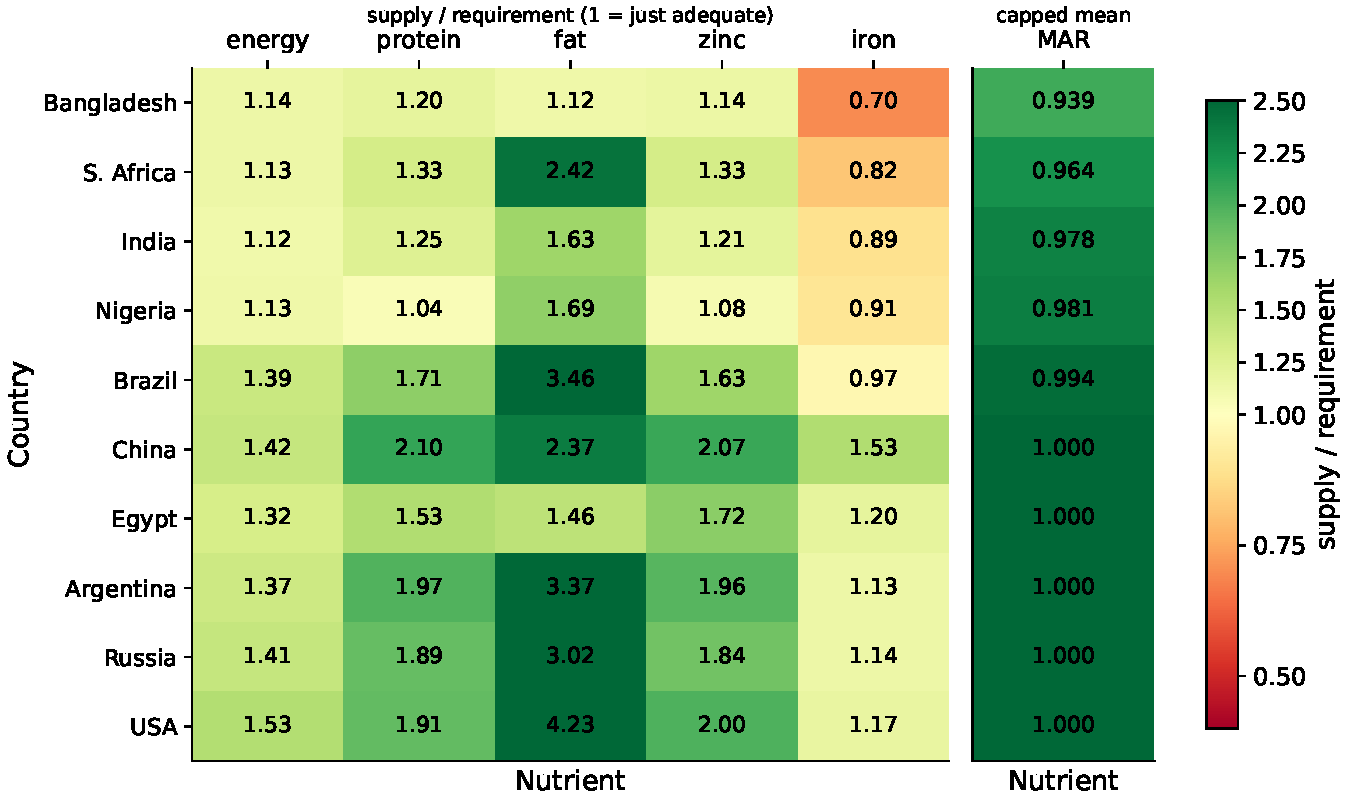
\includegraphics[width=\linewidth]{F07_adequacy_panel.pdf}
\caption{Nutrient adequacy (supply $\div$ requirement).}
\end{minipage}
\end{figure}
Wheat and rice provide the bulk of cereal protein, zinc, and iron worldwide (wheat supplies \worldProteinWheat\% of protein, \worldZincWheat\% of zinc, and \worldIronWheat\% of iron in panel countries). Soybean contributes primarily fat (\worldFatSoybean\%) as most is crushed for oil, while maize contributes modestly to direct human diets (\worldKcalMaize\% kcal) as the majority is used for animal feed.

\textbf{Iron is the binding nutritional constraint}: national supply relative to requirement is \feRatioBangladesh\ in Bangladesh, \feRatioSAfrica\ in South Africa, and \feRatioIndia\ in India, whereas energy and protein requirements are met at the national level.

\subsection{The Vulnerability Index}
\begin{figure}[H]\centering
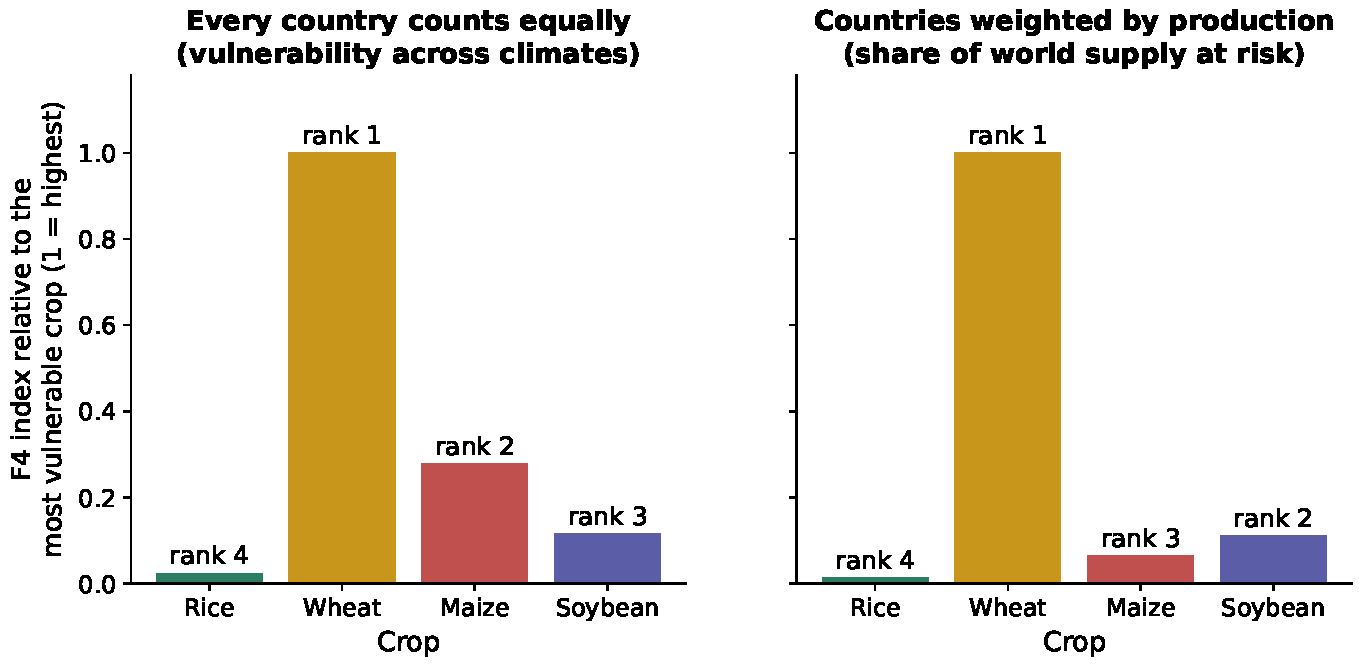
\includegraphics[width=0.85\linewidth]{F08s_index_F4.pdf}
\caption{F4 Vulnerability Index relative to the highest-scoring crop (1.0). Left: equal country weights; Right: production-weighted.}
\end{figure}

Under equal country weights, F4 ranks crop vulnerability as:
$$\textbf{\orderFour}$$
Under production weighting, the ordering is:
$$\textbf{\orderFourPw}$$

\begin{table}[H]\centering\small
\begin{tabular}{llrrrr}
\toprule
Form & Country weights & Rice & Wheat & Maize & Soybean\\
\midrule
F1 $E\cdot S\cdot I$ & equal & 0.001 (4) & 0.064 (1) & 0.021 (2) & 0.010 (3) \\
 & production & 0.001 (4) & 0.081 (1) & 0.006 (3) & 0.012 (2) \\
F2 $(E S I)^{1/3}$ & equal & 0.077 (4) & 0.366 (1) & 0.201 (2) & 0.192 (3) \\
 & production & 0.081 (4) & 0.407 (1) & 0.153 (3) & 0.207 (2) \\
F3 $(E+S+I)/3$ & equal & 0.229 (4) & 0.410 (1) & 0.318 (2) & 0.297 (3) \\
 & production & 0.283 (3) & 0.429 (1) & 0.242 (4) & 0.295 (2) \\
F4 paired $\times I$ & equal & 0.002 (4) & 0.065 (1) & 0.018 (2) & 0.008 (3) \\
 & production & 0.001 (4) & 0.084 (1) & 0.005 (3) & 0.009 (2) \\
\bottomrule
\end{tabular}

\caption{Crop vulnerability index under each candidate formula and weighting (rank in parentheses).}\label{tab:crop_index}
\end{table}

\begin{figure}[H]\centering
\begin{minipage}{0.58\textwidth}
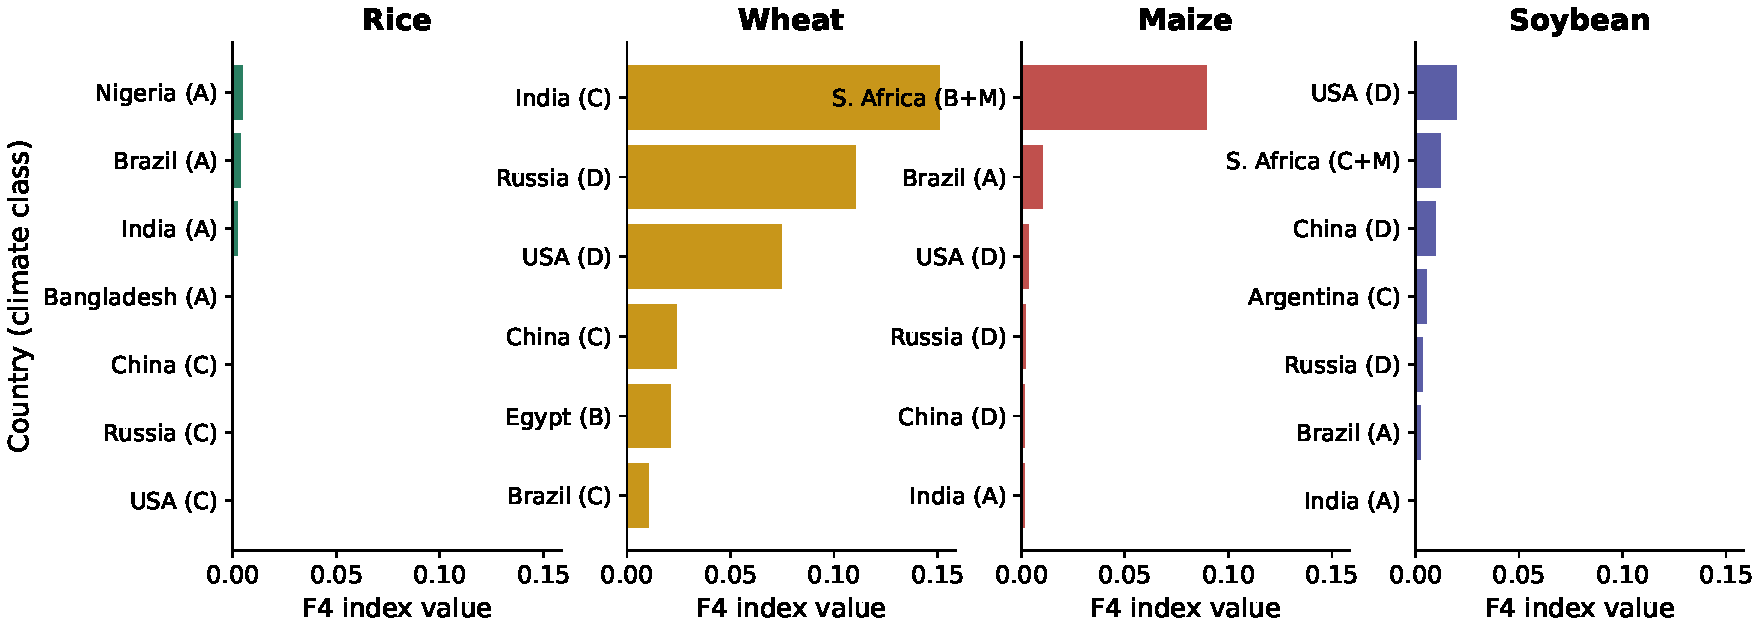
\includegraphics[width=\linewidth]{F09_country_index.pdf}
\caption{F4 vulnerability index by crop and country.}
\end{minipage}\hfill
\begin{minipage}{0.38\textwidth}
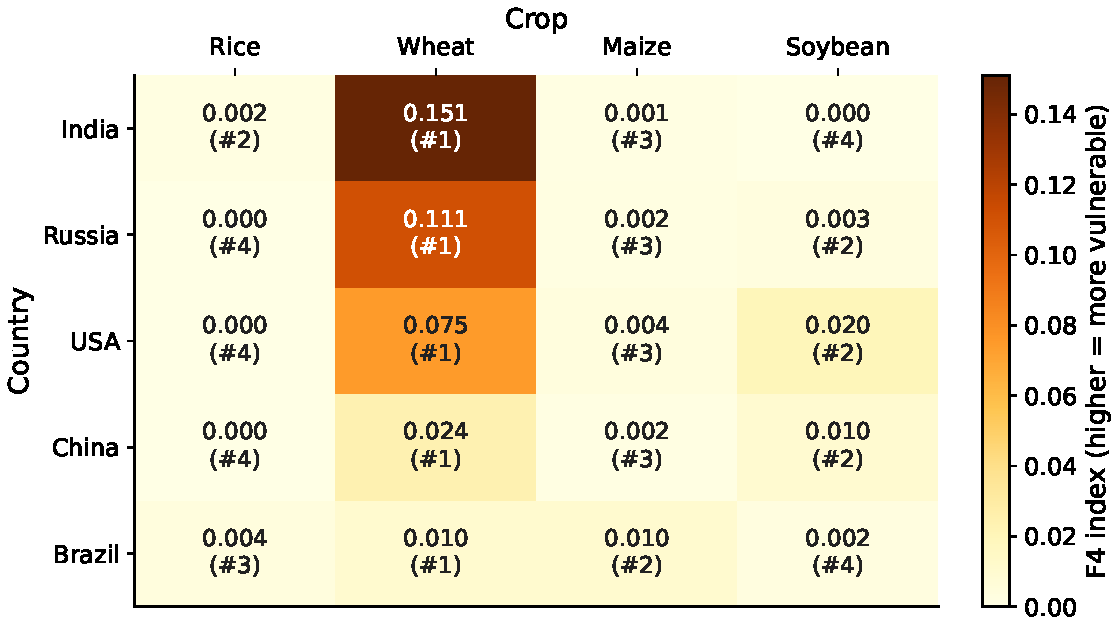
\includegraphics[width=\linewidth]{F17_country_crop_matrix.pdf}
\caption{Within-country crop vulnerability rank.}
\end{minipage}
\end{figure}

Wheat ranks \#1 across all \sharedWheatTop\ shared panel countries that grow all four crops, driven by the combination of high dietary dependence and substantial climate exposure in major producers (India $0.1511$, Russia $0.1105$, USA $0.0747$). Maize exhibits localized high vulnerability in South Africa ($0.0895$) where it is a primary dietary staple grown under rainfed conditions.

\begin{table}[H]\centering\small
\begin{tabular}{lcccc}
\toprule
\textbf{Country} & \textbf{Rice} & \textbf{Wheat} & \textbf{Maize} & \textbf{Soybean} \\
\midrule
USA & $<0.0001$ & 0.0747 & 0.0037 & 0.0197 \\
Brazil & 0.0039 & 0.0103 & 0.0103 & 0.0025 \\
India & 0.0023 & 0.1511 & 0.0015 & 0.0002 \\
China & 0.0001 & 0.0240 & 0.0016 & 0.0097 \\
Russia & $<0.0001$ & 0.1105 & 0.0021 & 0.0032 \\
Argentina & -- & -- & -- & 0.0052 \\
Bangladesh & 0.0002 & -- & -- & -- \\
Egypt & -- & 0.0209 & -- & -- \\
Nigeria & 0.0046 & -- & -- & -- \\
South Africa & -- & -- & 0.0895 & 0.0122 \\
\bottomrule
\end{tabular}

\caption{Country-by-crop F4 vulnerability index ($V_{F4}$).}\label{tab:country_crop_index}
\end{table}

\subsection{Robustness and Validation}
\paragraph{Robustness.} Evaluating 10 one-at-a-time modifications (scaling methods, weighting schemes, parameter proxies) across 4 formulas and 2 weighting types (\robN\ total permutations) confirms that \textbf{wheat ranks \#1 in \robWheatTopAll\ of \robN\ tests}. In Monte Carlo simulations with 2,000 random weight assignments, wheat ranks first in \mcFourWheatFirst\% of iterations under F4.

\paragraph{Validation.} 
- \emph{Zhao et al. (2017):} Full F4 index rank correlation with global warming yield declines is $\rho=\rhoZhaoFour$.
- \emph{Myers et al. (2014):} Elevated CO$_2$ declines disproportionately affect wheat and rice zinc and iron, aligning with our nutritional importance rankings.
- \emph{Yield shocks:} Observed 2001--2024 yield shocks show weak positive association ($\rho=\rhoShock, p=\pShock$) with the climate index.

\subsection{Yield to Diet Scenarios}
\begin{figure}[H]\centering
\begin{minipage}{0.49\textwidth}
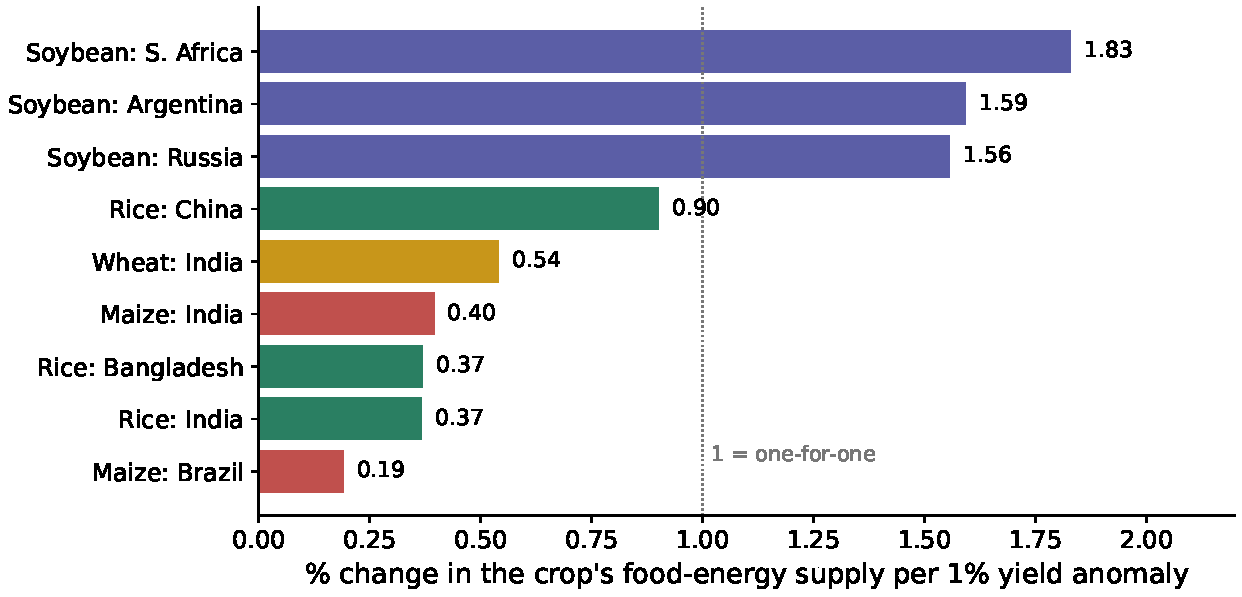
\includegraphics[width=\linewidth]{F13c_passthrough_clear.pdf}
\caption{Yield pass-through $\beta$ to food supply.}
\end{minipage}\hfill
\begin{minipage}{0.49\textwidth}
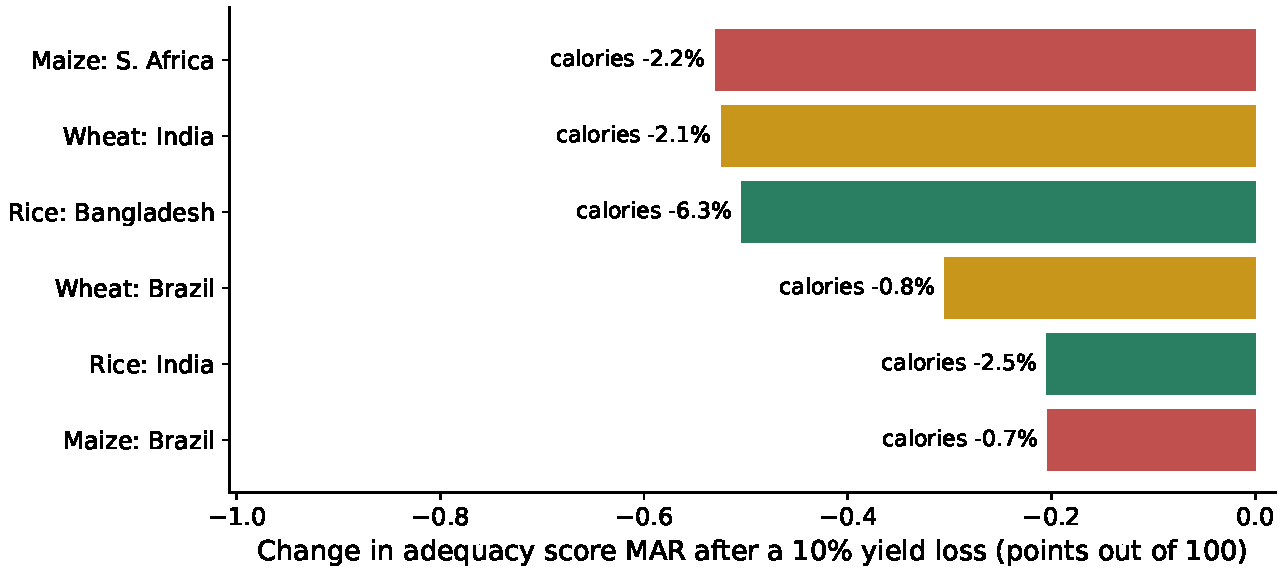
\includegraphics[width=\linewidth]{F14c_scenario_simple.pdf}
\caption{Fall in MAR following a 10\% yield loss.}
\end{minipage}
\end{figure}
A standard $-10\%$ yield loss reduces dietary adequacy most severely for maize in South Africa and wheat in India, where iron availability is already close to requirement levels.

% =====================================================================
\section{Conclusions}
\begin{enumerate}\setlength{\itemsep}{3pt}
\item \textbf{Wheat is the most vulnerable crop} to climate-driven nutritional disruption (\orderFour\ with equal weights; \orderFourPw\ production-weighted).
\item \textbf{Key drivers for wheat:} High dietary reliance for protein, zinc, and iron, coupled with high heat exposure in South Asia and moisture deficits in North America and Russia.
\item \textbf{Maize and soybean} have high intrinsic heat sensitivity, but lower direct food importance globally because they are predominantly utilized for feed and industrial processing.
\item \textbf{Rice scores lowest} due to widespread irrigation and monthly mean temperatures below \SI{35}{\celsius}, though localized short-duration heat spikes during flowering remain an uncaptured risk.
\item \textbf{Iron} is the primary binding nutrient constraint across developing country diets.
\end{enumerate}

\bibliography{refs}

\appendix


\section{Index Components and Scenario Data}\label{app:tables}
\begin{table}[H]\centering\tiny
\adjustbox{max width=\linewidth}{\begin{tabular}{llrrrrrrrrrr}
\toprule
 & & \multicolumn{2}{c}{Heat} & \multicolumn{2}{c}{Water} & \multicolumn{2}{c}{Exposure} & \multicolumn{2}{c}{Sensitivity} & & \\
\cmidrule(lr){3-4}\cmidrule(lr){5-6}\cmidrule(lr){7-8}\cmidrule(lr){9-10}
Crop & Country & $L$ (\si{\celsius}) & $\Delta$ (SD) & $L$ (\%) & $\Delta$ (SD) & $E_h$ & $E_w$ & $S_h$ & $S_w$ & $I$ (\%) & $V_{F4}$\\
\midrule
Rice & China (C) & 0.00 & 0.77 & 0.0 & 0.00 & 0.00 & 0.00 & 0.17 & 0.50 & 13.3 & 0.000 \\
 & India (A) & 0.00 & 1.05 & 1.3 & 0.00 & 0.00 & 0.02 & 0.66 & 0.50 & 15.6 & 0.002 \\
 & Bangladesh (A) & 0.00 & 0.87 & 0.1 & 0.12 & 0.00 & 0.00 & 0.17 & 0.50 & 42.1 & 0.000 \\
 & Brazil (A) & 0.00 & 1.08 & 7.6 & 0.06 & 0.00 & 0.14 & 0.17 & 0.50 & 4.7 & 0.004 \\
 & USA (C) & 0.00 & 0.46 & 0.0 & 0.00 & 0.00 & 0.00 & 0.33 & 0.50 & 1.2 & 0.000 \\
 & Nigeria (A) & 0.00 & 0.64 & 7.6 & 0.00 & 0.00 & 0.14 & 0.17 & 0.50 & 5.6 & 0.005 \\
 & Russia (C) & 0.00 & 1.58 & 0.2 & 0.00 & 0.00 & 0.00 & 0.17 & 0.50 & 0.9 & 0.000 \\
\midrule
Wheat & China (C) & 0.01 & 1.34 & 15.0 & 0.01 & 0.02 & 0.27 & 0.37 & 0.44 & 16.0 & 0.024 \\
 & India (C) & 0.58 & 0.90 & 17.8 & 0.02 & 1.00 & 0.33 & 0.43 & 0.44 & 22.2 & 0.151 \\
 & Russia (D) & 0.07 & 0.54 & 31.4 & 0.05 & 0.13 & 0.57 & 0.37 & 0.44 & 31.0 & 0.111 \\
 & USA (D) & 0.08 & 0.24 & 36.9 & 0.01 & 0.13 & 0.68 & 0.37 & 0.44 & 18.2 & 0.075 \\
 & Egypt (B) & 0.08 & 1.46 & 0.1 & 0.00 & 0.14 & 0.00 & 0.37 & 0.44 & 34.4 & 0.021 \\
 & Brazil (C) & 0.01 & 0.96 & 7.3 & 0.25 & 0.02 & 0.13 & 0.37 & 0.44 & 13.3 & 0.010 \\
\midrule
Maize & USA (D) & 0.01 & 0.38 & 16.3 & 0.00 & 0.02 & 0.30 & 0.46 & 0.50 & 2.0 & 0.004 \\
 & China (D) & 0.01 & 0.77 & 8.5 & 0.00 & 0.01 & 0.15 & 0.40 & 0.66 & 1.3 & 0.002 \\
 & Brazil (A) & 0.00 & 0.99 & 13.6 & 0.21 & 0.01 & 0.25 & 0.69 & 0.50 & 6.7 & 0.010 \\
 & India (A) & 0.04 & 0.85 & 3.7 & 0.00 & 0.06 & 0.07 & 0.69 & 0.50 & 1.6 & 0.001 \\
 & S. Africa (B+M) & 0.00 & 0.86 & 36.5 & 0.26 & 0.00 & 0.67 & 0.69 & 0.50 & 22.5 & 0.089 \\
 & Russia (D) & 0.00 & 1.20 & 54.6 & 0.48 & 0.00 & 1.00 & 0.69 & 1.00 & 0.2 & 0.002 \\
\midrule
Soybean & Brazil (A) & 0.00 & 1.08 & 3.8 & 0.13 & 0.00 & 0.07 & 0.76 & 0.42 & 7.3 & 0.002 \\
 & USA (D) & 0.00 & 0.35 & 22.3 & 0.00 & 0.00 & 0.41 & 0.67 & 0.42 & 9.7 & 0.020 \\
 & Argentina (C) & 0.00 & 0.55 & 26.1 & 0.19 & 0.00 & 0.48 & 0.76 & 0.61 & 1.5 & 0.005 \\
 & China (D) & 0.00 & 0.71 & 13.8 & 0.00 & 0.00 & 0.25 & 0.76 & 0.56 & 5.8 & 0.010 \\
 & India (A) & 0.00 & 0.59 & 0.9 & 0.00 & 0.00 & 0.02 & 0.76 & 0.42 & 2.4 & 0.000 \\
 & Russia (D) & 0.00 & 0.63 & 32.5 & 0.09 & 0.00 & 0.60 & 0.76 & 0.42 & 1.1 & 0.003 \\
 & S. Africa (C+M) & 0.00 & 0.83 & 35.4 & 0.33 & 0.00 & 0.65 & 0.76 & 0.42 & 3.8 & 0.012 \\
\bottomrule
\end{tabular}
}
\caption{Detailed index components by crop and country.}
\end{table}

\begin{table}[H]\centering\tiny
\adjustbox{max width=\linewidth}{\begin{tabular}{llrrrrrrr}
\toprule
 & & & \multicolumn{2}{c}{Climate-driven $\Delta Y$ (\%)} & \multicolumn{4}{c}{Standard $-10$\% yield shock (S3)}\\
\cmidrule(lr){4-5}\cmidrule(lr){6-9}
Crop & Country & SSR & S1 shift & S2 1-in-10 & $\Delta$kcal\% & $\Delta$Zn\% & $\Delta$Fe\% & $\Delta$MAR pts (no trade / trade)\\
\midrule
Rice & China & 0.95 & +0.0 & +0.0 & -2.36 & -1.51 & -0.82 & +0.00 / +0.00\\
 & India & 1.19 & -4.8 & -3.3 & -2.47 & -2.09 & -1.15 & -0.20 / -0.00\\
 & Bangladesh & 1.02 & +0.0 & +0.0 & -6.29 & -5.45 & -3.62 & -0.50 / -0.51\\
 & Brazil & 1.04 & +0.0 & +0.0 & -0.78 & -0.59 & -0.40 & -0.08 / +0.00\\
 & USA & 1.43 & -1.4 & -2.7 & -0.21 & -0.15 & -0.11 & +0.00 / +0.00\\
 & Nigeria & 1.00 & +0.0 & +0.0 & -0.83 & -0.76 & -0.37 & -0.07 / -0.07\\
 & Russia & 0.79 & +0.0 & +0.0 & -0.12 & -0.09 & -0.06 & +0.00 / +0.00\\
\midrule
Wheat & China & 0.90 & -3.7 & -4.0 & -1.62 & -1.92 & -1.72 & +0.00 / +0.00\\
 & India & 1.01 & -3.2 & -4.1 & -2.11 & -3.26 & -2.95 & -0.52 / -0.28\\
 & Russia & 1.78 & -3.1 & -4.8 & -2.91 & -4.56 & -4.90 & +0.00 / +0.00\\
 & USA & 1.25 & -1.1 & -4.8 & -1.54 & -2.72 & -3.09 & +0.00 / +0.00\\
 & Egypt & 0.56 & -3.6 & -3.3 & -1.90 & -2.70 & -2.57 & +0.00 / +0.00\\
 & Brazil & 0.69 & +1.1 & -16.8 & -0.75 & -1.41 & -1.57 & -0.31 / +0.00\\
\midrule
Maize & USA & 1.20 & -2.8 & -4.6 & -0.21 & -0.29 & -0.33 & +0.00 / +0.00\\
 & China & 0.92 & -2.8 & -4.4 & -0.15 & -0.16 & -0.14 & +0.00 / +0.00\\
 & Brazil & 1.55 & -7.0 & -6.1 & -0.72 & -0.92 & -1.05 & -0.20 / +0.00\\
 & India & 1.15 & -4.6 & -2.7 & -0.18 & -0.23 & -0.21 & -0.04 / -0.00\\
 & S. Africa & 1.36 & -26.8 & -23.8 & -2.17 & -2.95 & -3.23 & -0.53 / -0.00\\
 & Russia & 1.28 & -38.1 & -31.4 & -0.02 & -0.03 & -0.03 & +0.00 / +0.00\\
\midrule
Soybean & Brazil & 2.52 & -4.3 & -4.3 & -0.98 & -0.00 & -0.01 & -0.00 / +0.00\\
 & USA & 1.65 & -0.8 & -3.9 & -1.43 & -0.00 & -0.01 & +0.00 / +0.00\\
 & Argentina & 0.97 & -4.6 & -16.9 & -0.20 & -0.00 & -0.00 & +0.00 / +0.00\\
 & China & 0.27 & -2.6 & -7.6 & -0.10 & -0.08 & -0.18 & +0.00 / +0.00\\
 & India & 0.82 & +0.8 & -8.9 & -0.17 & -0.01 & -0.03 & -0.01 / -0.01\\
 & Russia & 1.02 & -4.4 & -4.9 & -0.13 & -0.00 & -0.01 & +0.00 / +0.00\\
 & S. Africa & 1.13 & -7.1 & -6.6 & -0.43 & -0.03 & -0.09 & -0.01 / -0.00\\
\bottomrule
\end{tabular}
}
\caption{Yield-to-diet shock scenario results.}
\end{table}

\end{document}
